%% 
%% Copyright 2007-2020 Elsevier Ltd
%% 
%% This file is part of the 'Elsarticle Bundle'.
%% ---------------------------------------------
%% 
%% It may be distributed under the conditions of the LaTeX Project Public
%% License, either version 1.2 of this license or (at your option) any
%% later version.  The latest version of this license is in
%%    http://www.latex-project.org/lppl.txt
%% and version 1.2 or later is part of all distributions of LaTeX
%% version 1999/12/01 or later.
%% 
%% The list of all files belonging to the 'Elsarticle Bundle' is
%% given in the file `manifest.txt'.
%% 

%% Template article for Elsevier's document class `elsarticle'
%% with numbered style bibliographic references
%% SP 2008/03/01
%%
%% 
%%
%% $Id: elsarticle-template-num.tex 190 2020-11-23 11:12:32Z rishi $
%%
%%
\documentclass[preprint,12pt]{elsarticle}

%% Use the option review to obtain double line spacing
%% \documentclass[authoryear,preprint,review,12pt]{elsarticle}

%% Use the options 1p,twocolumn; 3p; 3p,twocolumn; 5p; or 5p,twocolumn
%% for a journal layout:
%% \documentclass[final,1p,times]{elsarticle}
%% \documentclass[final,1p,times,twocolumn]{elsarticle}
%% \documentclass[final,3p,times]{elsarticle}
%% \documentclass[final,3p,times,twocolumn]{elsarticle}
%% \documentclass[final,5p,times]{elsarticle}
%% \documentclass[final,5p,times,twocolumn]{elsarticle}

%% For including figures, graphicx.sty has been loaded in
%% elsarticle.cls. If you prefer to use the old commands
%% please give \usepackage{epsfig}

%% The amssymb package provides various useful mathematical symbols
\usepackage{amssymb}
\usepackage{multirow}
\usepackage{lineno}
\usepackage[colorlinks,citecolor=black,linkcolor=black,urlcolor=black,bookmarks,bookmarksnumbered]{hyperref}
%% The amsthm package provides extended theorem environments
\usepackage{amsthm}
\usepackage{amsmath}

%% The lineno packages adds line numbers. Start line numbering with
%% \begin{linenumbers}, end it with \end{linenumbers}. Or switch it on
%% for the whole article with \linenumbers.
%% \usepackage{lineno}

\journal{Energy}

\begin{document}

\begin{frontmatter}

%% Title, authors and addresses

%% use the tnoteref command within \title for footnotes;
%% use the tnotetext command for theassociated footnote;
%% use the fnref command within \author or \address for footnotes;
%% use the fntext command for theassociated footnote;
%% use the corref command within \author for corresponding author footnotes;
%% use the cortext command for theassociated footnote;
%% use the ead command for the email address,
%% and the form \ead[url] for the home page:
%% \title{Title\tnoteref{label1}}
%% \tnotetext[label1]{}
%% \author{Name\corref{cor1}\fnref{label2}}
%% \ead{email address}
%% \ead[url]{home page}
%% \fntext[label2]{}
%% \cortext[cor1]{}
%% \affiliation{organization={},
%%             addressline={},
%%             city={},
%%             postcode={},
%%             state={},
%%             country={}}
%% \fntext[label3]{}

\title{Self-tunable approximated explicit MPC: Heat exchanger implementation}
%\title{Self-tunable approximated explicit MPC: Implementation on a heat exchanger with a non-symmetric behavior}

%% use optional labels to link authors explicitly to addresses:
%% \author[label1,label2]{}
%% \affiliation[label1]{organization={},
%%             addressline={},
%%             city={},
%%             postcode={},
%%             state={},
%%             country={}}
%%
%% \affiliation[label2]{organization={},
%%             addressline={},
%%             city={},
%%             postcode={},
%%             state={},
%%             country={}}

\author{Lenka Galčíková}
\author{Juraj Oravec}
\author{Petronela Belková}

\affiliation{organization={Slovak University of Technology in Bratislava, Faculty of Chemical and Food Technology, Institute of Information Engineering, Automation, and Mathematics,},%Department and Organization
            addressline={Radlinského 9}, 
            city={Bratislava},
            postcode={81237}, 
%            state={Slovakia},
            country={Slovakia}
}

\begin{abstract}
max 250 words!

\end{abstract}

%%Graphical abstract
\begin{graphicalabstract}
%\includegraphics{grabs}
\end{graphicalabstract}

%%Research highlights
\begin{highlights}
\item Research highlight 1
\item Research highlight 2
\end{highlights}

\begin{keyword}
%% keywords here, in the form: keyword \sep keyword

%% PACS codes here, in the form: \PACS code \sep code

%% MSC codes here, in the form: \MSC code \sep code
%% or \MSC[2008] code \sep code (2000 is the default)

\end{keyword}

\end{frontmatter}

%% \linenumbers

%% main text
\section{Introduction}
\label{sec:introduction}
 
(skor intro?)The benefit in form of lower computational complexity in the control phase comes hand in hand with a drawback. The size of the parametric solution may be so large, that it becomes impractical to utilize for two reasons: (i) memory footprint is higher than the available memory size of the control unit, (ii) the computational time associated with finding the optimal control action is higher than the available time period for control action implementation. Although this control strategy has its challenges, it is still very beneficial for practical usage for its benefits. 

\section{Preliminaries}
\label{sec:preliminaries}
In this section, the theoretical background necessary for this work is summarized. First, the explicit model predictive control is recalled. Next, the tunable technique of the approximated explicit model predictive control is introduced. Last but not least, the self-tunable technique of the approximated explicit MPC is presented.

\subsection{Explicit model predictive control}
\label{sec:eMPC}
TODO: remark, ze sme si vedomi aj delta-u formulacie, ale vedie na zlozitejsie eMPC

Explicit model predictive control~\cite{Bemporad_automatica} represents a parametric solution of the model predictive control which makes it suitable for online implementation. As the explicit solution is available, it is not necessary to solve the optimization problem in every control step. As this work deals with practical implementation, let us consider the optimization problem in the following form:

\begin{subequations}
	\label{eq:mpc_problem}
	\begin{eqnarray}
		\label{eq:mpc_problem_cost}
		\min_{u_0,u_{1},\ldots,u_{N-1}} &~& \! \sum_{k=0}^{N-1} \! \left( (y_k-y_\mathrm{ref})^{\intercal} Q_\mathrm{y} (y_k-y_\mathrm{ref}) + u_{k}^{\intercal} R u_{k} + x_{\mathrm{I},k}^{\intercal} Q_\mathrm{x} x_{\mathrm{I},k} \right)  \\
		\label{eq:mpc_problem_prediction_model_x}
		\mathrm{s.t.\!:} &~& \widetilde{x}_{k+1} = \widetilde{A}\,\widetilde{x}_{k} + \widetilde{B}\,u_{k}, \\
		\label{eq:mpc_problem_prediction_model_y}
		&~& y_{k} = \widetilde{C}\,\widetilde{x}_{k}, \\
		\label{eq:mpc_problem_input_constraints}
		&~& u_{k} \in \mathcal{U}, \\
		\label{eq:mpc_problem_state_constraints}
		&~& y_{k} \in \mathcal{Y}, \\
		\label{eq:mpc_problem_initial_coindition}
		&~& \widetilde{x}_{0} = \theta, \\
		\label{eq:mpc_problem_k_range}
		&~& k = 0,1,\ldots, N-1,
	\end{eqnarray}
\end{subequations}

where $k$ denotes the step of the prediction horizon $N$. The parameter $\theta \in \Theta$ in Eq.~\eqref{eq:mpc_problem_initial_coindition} represents the initial condition of the optimization problem for which it is parametrically precomputed. The prediction model in~\eqref{eq:mpc_problem_prediction_model_x}--\eqref{eq:mpc_problem_prediction_model_y} has the form of extended linear time-invariant (LTI) system for given extended state matrix $\widetilde{A} \in \mathbb{R}^{n_{\mathrm{x}} \times n_{\mathrm{x}}}$, extended input matrix $\widetilde{B} \in \mathbb{R}^{n_{\mathrm{x}} \times n_{\mathrm{u}}}$ and extended output matrix $\widetilde{C} \in \mathbb{R}^{n_{\mathrm{y}} \times n_{\mathrm{x}}}$. Variables $\widetilde{x} \in \mathbb{R}^{n_{\mathrm{x}}}$, $u \in \mathbb{R}^{n_{\mathrm{u}}}$, $y \in \mathbb{R}^{n_{\mathrm{y}}}$ are vectors of corresponding extended system states, control inputs and system outputs, respectively. The sets $\mathcal{U} \subseteq \mathbb{R}^{n_{\mathrm{u}}}$, $\mathcal{Y} \subseteq \mathbb{R}^{n_{\mathrm{x}}}$ are sets of physical constraints on inputs and outputs, respectively. The penalty matrix $Q_\mathrm{y} \in \mathbb{R}^{n_{\mathrm{y}} \times n_{\mathrm{y}}}$ penalizes the squarred control error, i.e., the deviation between the output and output reference value $y_\mathrm{ref}$. The matrix $R \in \mathbb{R}^{n_{\mathrm{u}} \times n_{\mathrm{u}}}$ penalizes the squarred value of control inputs. To obtain the offset-free control results, the built-in integrator was included in the state-space model, see e.q.~\cite{Ruscio_MPC_integral}. The value of integrator is also penalized in the cost function with the penalty matrix $Q_\mathrm{x} \in \mathbb{R}^{n_{\mathrm{y}} \times n_{\mathrm{y}}}$.

The model extended with the built-in integrator in~\eqref{eq:mpc_problem_prediction_model_x}--\eqref{eq:mpc_problem_prediction_model_y} can be rewritten as:

\begin{subequations}
	\begin{eqnarray} 
		\label{eq:mpc_extended_model_x} 
		\widetilde{x}_{k+1} &=& \begin{bmatrix} x_{k+1} \\ 	x_{\mathrm{I},k+1}\end{bmatrix} = \begin{bmatrix} A & \textit{0} \\ -T_\mathrm{s} C & I \end{bmatrix} \begin{bmatrix} x_{k} \\ x_{\mathrm{I},k} \end{bmatrix} + \begin{bmatrix} B \\ I \end{bmatrix} u_{k}, \\
		\label{eq:mpc_extended_model_y}
		y_k &=& \begin{bmatrix} C & \textit{0} \end{bmatrix} \begin{bmatrix} x_{k} \\ x_{\mathrm{I},k} \end{bmatrix},
	\end{eqnarray}
\end{subequations}

where $x_{\mathrm{I}} \in \mathbb{R}^{n_{\mathrm{y}}}$ is the integral of the control error, $T_\mathrm{s}$ denotes the sampling time and matrices $A$, $B$, $C$ are well-known linear time-invariant state-space matrices that form the extended model. Thanks to this extension and penalization in the cost function in Eq.~\eqref{eq:mpc_problem_cost}, not only the control error are penalized, but also its integral, which leads to similar results as incorporating integral part in PID controller.

Solving the MPC quadratic optimization problem in Eq.~\eqref{eq:mpc_problem} parametrically leads to explicit solution in the form of piece-wise affine control law consisting of $r$ critical regions:

\begin{eqnarray}
\label{eq:PWA_control_law}
u(\theta) = \left\{ 
\begin{matrix}
	F_{1} \, \theta + g_{1} & \mathrm{if} & \quad \theta \in \mathcal{R}_1, \\
	F_{2} \, \theta + g_{2} & \mathrm{else}\,\,\mathrm{if} &\quad \theta \in \mathcal{R}_2, \\
	\vdots & \\
	F_{r} \, \theta + g_{r} & \mathrm{else}\,\,\mathrm{if} & \quad \theta \in \mathcal{R}_{r}, \\
\end{matrix}
\right.
\end{eqnarray}
where $F_{i}$ and $g_{i}$ respectively are the slope and affine section of the corresponding control law. The piece-wise affine function from Eq.~\eqref{eq:PWA_control_law} is stored and used in the online, i.e., control phase. Based on identifying the critical region where the parameter $\theta$ belongs, the optimal control input is calculated based on the associated control law.

Note, many other formulations of the optimization problems are elaborated, mainly in the terms of cost functions. Also, the incremental (velocity) formulation of the state-space model is common, but leads to further extendsion of the vector of parameters $\theta$ and therefore the explicit MPC complexity increases. Another option for offset-free tracking is also disturbance observer. For such an overview see e.g. ...TODO. 
Klauco reference governors? minimovka zdroje



      

\subsection{Tunable explicit model predictive control}
\label{sec:tunable}

\subsection{Self-tunable explicit model predictive control}
\label{sec:self_tunable}


\section{Methodology}
\label{sec:methodology}

\subsection{Self-tunable technique for systems with asymmetric behavior}
\label{sec:self_tunable_new}

TODO: spomenut, ze to je vhodne celkovo aj pre klasicke online MPC

\section{Results and discussion}
\label{sec:results}

In this section, the results of the proposed tuning method are presented. The plant on which the control was implemented is a laboratory liquid-to-liquid plate heat exchanger Armfield Process Plant Trainer PCT23~\cite{pct23}, see Fig.~\ref{fig:HE}. The cold feed as well as heating medium are transported to the heat exchanger by two peristaltic pumps. The flow rate of the feed is constant, while the aim is to track the reference value of its temperature. Therefore, the controlled variable is the feed temperature $T$ at the outlet of the heat exchanger and the manipulated variable is the voltage $U$ corresponding to the power of the heating medium pump. The voltage is set in percentage, while it is constrained from 20\% to 100\%. As the heat exchange is a nonlinear and non-symmetric process~\cite{Liptak}, this heat exchanger represents a suitable candidate for the presented controller tuning strategy.  

The matrices of the linear state-space model of the plant, discretized with sampling time $T_\mathrm{s}$ = 1\,s, are

\begin{subequations}
	\label{eq:model_A_B} 
	\begin{eqnarray}
		A&=&\begin{bmatrix}
			0.839
		\end{bmatrix}, \\
		B&=&\begin{bmatrix}
			0.039
		\end{bmatrix}, \\
		C&=&\begin{bmatrix}
			1
		\end{bmatrix}, \\
		D&=&\begin{bmatrix}
			0
		\end{bmatrix}.
		\end{eqnarray}
\end{subequations}

The constraints are considered in the terms of manipulated variable, i.e.

\begin{eqnarray}
\label{eq:u_const}
	-15\% \le u \le 65\%.
\end{eqnarray}

Note, the variable $u$ represents the manipulated variable in the deviation form. The values of feed temperature and voltage of the heating medium pump corresponding to zero steady state are respectively $T^\mathrm{s}$~=~35 $^{\circ}\mathrm{C}$ and $U^\mathrm{s}$~=~35\%.

The penalty matrices of the problem Eq.~\eqref{eq:mpc_problem} were systematically tuned and the corresponding control was implemented on the laboratory heat exchanger for every MPC setup. The aim was to determine, which penalty matrix will be the tuned one. Based on observations, the most significant effect on the control trajectories had tuning the penalty matrix $Q_\mathrm{y}$, while still preserving a satisfactory control performance, i.e., without steady-state control error and significant oscillations around the setpoint. The boundary values of matrix $Q_\mathrm{y}$ were tuned as $Q_\mathrm{y, L}$ = 100 and $Q_\mathrm{y, U}$ = 1000. The built-in integrator was penalized with $Q_\mathrm{x2}$ = 1 and the manipulated variable with $R$ = 10. The prediction horizon $N$ was 20 steps long. The explicit model predictive controllers were constructed in MATLAB R2020b using the Multi-Parametric Toolbox 3~\cite{mpt_conf}. 
The controllers were implemented to track a time-varying reference. For the first 200 seconds, the system was in the steady state. After that the reference changed its value twice upwards and twice downwards. The reference changes also acquired different sizes in order to examine the proposed tuning method as it is dependent on the size of the reference step change. The control results for both control setups are compared in Fig.~\ref{fig:CV_boundaries} for the controlled variable, and in Fig.~\ref{fig:MV_boundaries} for the manipulated variable.
    

\begin{figure}
	\begin{center}
		\includegraphics[width=0.8\textwidth]{images/HE}
		\caption[Heat exchanger Armfield Process Plant Trainer PCT23]{Laboratory heat exchanger Armfield Process Plant Trainer PCT23: feed pump\,(1), heating medium pump\,(2), feed tanks\,(3), heater for heating medium\,(4), heat exchanger\,(5).}
		\label{fig:HE}
	\end{center}
\end{figure}

\begin{figure}
	\begin{center}
		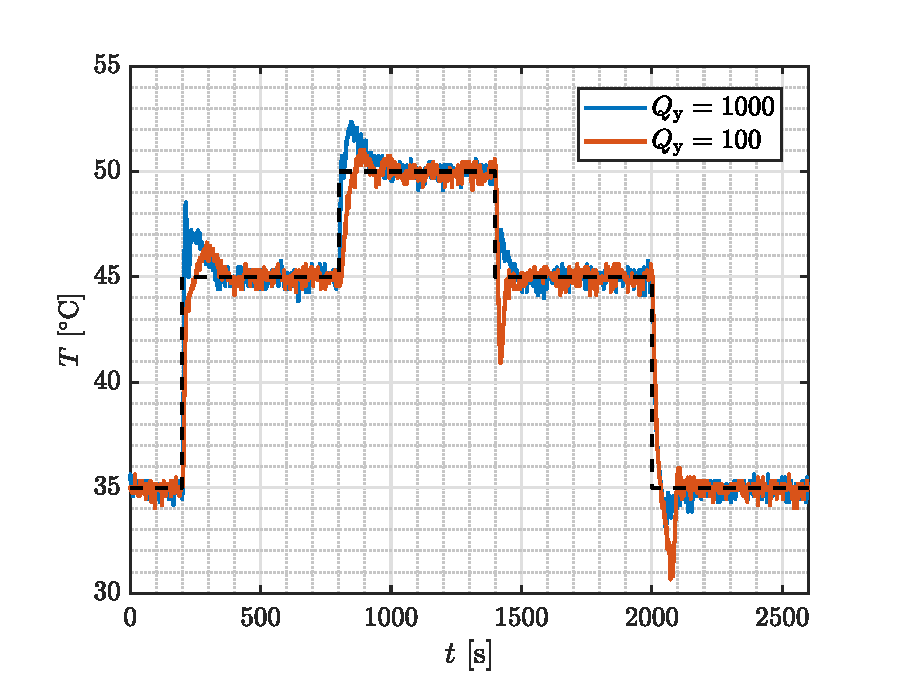
\includegraphics[width=0.8\textwidth]{images/CV_boundaries}
		\caption{Controlled variable trajectory for two boundary controllers. The solid lines represent the controlled temperature and the dashed line represents the reference value.}
		\label{fig:CV_boundaries}
	\end{center}
\end{figure}

\begin{figure}
	\begin{center}
		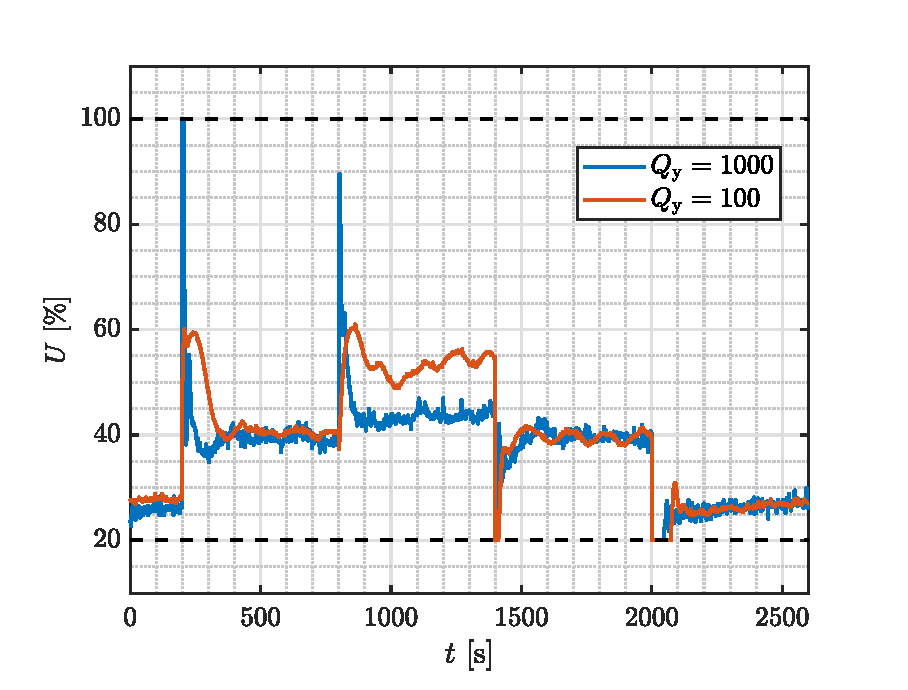
\includegraphics[width=0.8\textwidth]{images/MV_boundaries}
		\caption{Manipulated variable trajectory for two boundary controllers. The solid lines represent the voltage and the dashed lines represent the constraints.}
		\label{fig:MV_boundaries}
	\end{center}
\end{figure}

The trajectories in Fig.~\ref{fig:CV_boundaries} show the non-symmetric nature of controlling the process of heat exchange mainly when observing the overshoots and undershoots. When applying the control associated with the lower bound $Q_\mathrm{y, L}$, significant undershoots are present when tracking the reference downwards, i.e., when the reference change is negative. On the contrary, when implementing the controller associated with $Q_\mathrm{y, U}$, the undershoots are negligible, but significant overshoots can be seen when tracking the reference upwards.

These observations form the base for the strategy of self-tuning the penalty matrix $Q_\mathrm{y}$. The strategy follows the ideas summarized in Section~\ref{sec:self_tunable_new}.

TODO: dopisat strucne princip ladenia podla toho, ako bude spisana teoria v ~\ref{sec:self_tunable_new}. odkazat sa na rovnice atd...

The control results of the selt-tunable technique compared to the boundary controllers can be seen in Fig.~\ref{fig:CV} for the controlled variable, and in Fig.~\ref{fig:MV} for the manipulated variable. It can be seen that the tuned controller combined the benefits of the two boundary controllers. The overshoots and undershoots were reduced, as in the first half of control the penalty matrix $Q_\mathrm{y}$ acquired value from the first half of the penalty interval. When tracking the reference with negative change, the penalty matrix acquired the values from the second half of the interval, i.e., closer to the upper bound $Q_\mathrm{y,U}$. 
The similarity with the boundary controllers can be seen also on the manipulated variable trajectory. Note, the constraints on the input variable were satisfied as they were scaled based on the boundary controllers which are constructed considering the contraints. 

TODO: what about state constraints?


\begin{figure}
	\begin{center}
		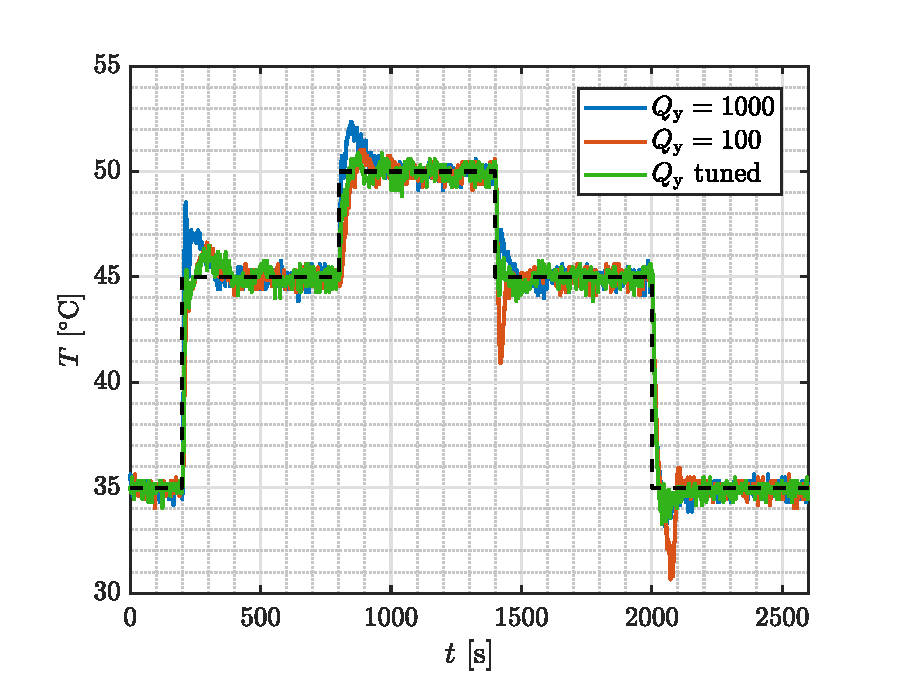
\includegraphics[width=0.8\textwidth]{images/CV}
		\caption{Controlled variable trajectory for two boundary controllers and the tuned one. The solid lines represent the controlled temperature and the dashed line represents the reference value.}
		\label{fig:CV}
	\end{center}
\end{figure}

\begin{figure}
	\begin{center}
		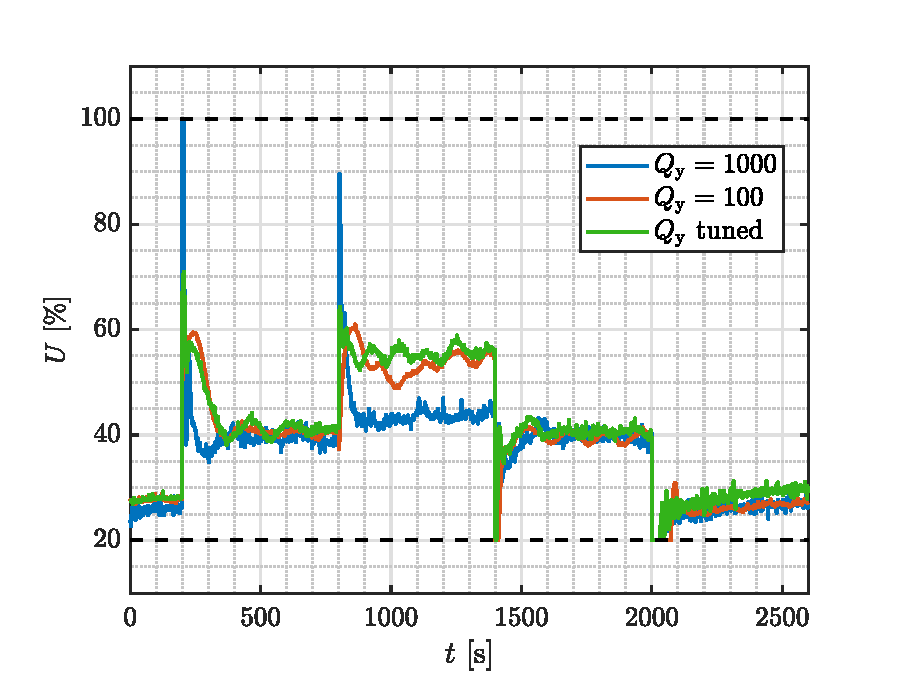
\includegraphics[width=0.8\textwidth]{images/MV}
		\caption{Manipulated variable trajectory for two boundary controllers and the tuned one. The solid lines represent the voltage and the dashed lines represent the constraints.}
		\label{fig:MV}
	\end{center}
\end{figure}

The control performance was also investigated quantitatively. The Table~\ref{tab:control_performance} summarizes the evaluated control performance criteria for the tuned and two boundary controllers. The control performance is evaluated for every reference step change respectively. The criteria are integral square error $ISE$, maximal overshoot/undershoot $\sigma_{\mathrm{max}}$, settling time $t_{\epsilon}$ for 5\%-neighbourhood of the reference value, and the volume of the heating medium utilized for the corresponding control. To provide better readability of the results, the best (i.e. minimal) values are written in bold. 

\begin{table}[h!]
	\begin{center}
		\caption{Control performance criteria.}
		\label{tab:control_performance}
		\begin{tabular}{c|c|c|c|c|c} 
			Reference step change & $Q_\mathrm{y}$ & $ISE$ [$^{\circ}\mathrm{C}^2$\,s] & $\sigma_{\mathrm{max}}$\,[\%] & $t_{\epsilon}$\,[s] & $V$\,[l] \\
			\hline
			\multirow{2}{*}{1} & 1000 & 714 & 33.50 & 16.5 & \textbf{2.12} \\
			    & 100 & 867 & 16.65 & 12.5 & 2.36 \\ 
			    & tuned & \textbf{678} & \textbf{15.19} & \textbf{9.5} & 2.38 \\ 
			\hline
			\multirow{2}{*}{2} & 1000 & 365 & 47.20 & \textbf{5} & \textbf{2.49} \\
			    & 100 & 606 & 23.25 & 26.5 & 3.19 \\ 
			    & tuned & \textbf{248} & \textbf{19.13} & 9.5 & 3.35 \\ 
			\hline
		    \multirow{2}{*}{3} & 1000 & 245 & \textbf{18.92} & \textbf{6.5} & \textbf{2.00} \\
				& 100 & 398 & 79.64 & 31 & \textbf{2.00} \\ 
				& tuned & \textbf{186} & 24.59 & \textbf{6.5} & 2.10 \\ 
			\hline
			\multirow{2}{*}{4} & 1000 & 1024 & 18.43 & 22.5 & 0.94 \\
				& 100 & 1402 & 41.87 & 90 & \textbf{0.93} \\ 
				& tuned & \textbf{967} & \textbf{16.49} & \textbf{18.5} & 1.10  
		\end{tabular}
	\end{center}
\end{table}

It can be seen in Table~\ref{tab:control_performance}, that real-time tuning of the controller helped to improve two to three criteria when tracking each reference value. The cost for this is the energy associated with control. Although the integral square error, maximal overshoot/undershoot and settling time decreased, the volume of consumed heating medium did not. Nevertheless, the average deterioration in the terms of consumed heating medium is approximately 17\%. 

The improvement or deterioration in percentage of using the tunable controller relative to the second best setup is summarized in Table~\ref{tab:improvement} for every reference step change separately. The negative numbers represent deterioration compared to the best controller setup in the corresponding reference tracking. 

\begin{table}[h!]
	\begin{center}
		\caption{Improvement or deterioration of the control performance in percentage.}
		\label{tab:improvement}
		\begin{tabular}{c|c|c|c|c} 
			Reference step change & $ISE$ & $\sigma_{\mathrm{max}}$ & $t_{\epsilon}$ & $V$ \\
			\hline
			1 & 5.04 & 8.77 & 24.00 & -12.26 \\ 
			\hline
			2 & 32.05 & 17.72 & -90.00 & -34.54 \\ 
			\hline
			3 & 24.08 & -29.97 & 0 & -4.48 \\ 
			\hline
			4 & 5.57 & 10.53 & 17.78 & -18.28  
		\end{tabular}
	\end{center}
\end{table}

It can be seen that implementing a tunable controller leads to improved control performance in many criteria. Utilizing a controller with a scalable aggressivity according to the operating conditions leads in general to higher accuracy, lower overshoot and faster achieving the reference value. %It should be also noted that the deterioration of every criterium is calculated subject to the best out of \textit{two} other controllers. It follows that the evaluation is strict as in practice only one controller would be available.
Although the volume of the heating medium is not saved in this control scenario, the improved control performance may lead to other benefits. 
TODO: krajsie skomentovat vyhody zlepsenia kvality riadenia

\section{Conclusion}
\label{sec:conclusion}


%% The Appendices part is started with the command \appendix;
%% appendix sections are then done as normal sections
%% \appendix

%% \section{}
%% \label{}

%% If you have bibdatabase file and want bibtex to generate the
%% bibitems, please use
%%

\bibliographystyle{elsarticle-num} 
\bibliography{references}

%% else use the following coding to input the bibitems directly in the
%% TeX file.

%\begin{thebibliography}{00}
%
%%% \bibitem{label}
%%% Text of bibliographic item
%
%\bibitem{}
%
%\end{thebibliography}

\end{document}
\endinput
%%
%% End of file `elsarticle-template-num.tex'.
